
The enclosure was difficult to construct for multiple reasons.  In order to
minimize the size of the PCB, we decided to forgo traditional mounting holes.
Additionally, we avoided using adhesive to mount the PCB in order to maintain
easy access for debugging and repair purposes.  This means the enclosure needed
tight tolerances around the PCB to prevent horizontal and vertical movement.
Additionally, the sensors mounted on the bottom of the PCB need to be a precise
distance away from the users wrist.  This means the thickness of the bottom of
the enclosure needed to be accurately tuned.

To add difficulty to the situation, the enclosure was manufactured by a (rather
cheap) desktop FDM 3D printer.  These printers are known for over extruding
plastic which causes the produced part to be slightly larger in the X and Y
dimensions.  As over extruding is preferable to under extruding (which weakens
the structural integrity of the part), it is common to simply model the part
slightly smaller to compensate.

FDM printers also tend to warp parts if the plastic cools too quickly, but that
can be countered by simply putting the printer in a warm room or giving the
printer a cozy blanket (although that is a fire hazard).

However, FDM 3D printing is exceptionally fast.  They make it possible to
iterate and print a 3D model of this size multiple times per day.  This rapid
iteration has enabled us to create parts that meet the above requirements.

The need for rapid iteration has led to the creation of many parametric 3D
modeling programs.  The idea is to define variables (like the the thickness of
the bottom of the model) that can easily be changed.  The problem with many of
these modeling programs is that they simply save a series of steps the user has
entered with the GUI so they can later replay this with different values.  This
replay of events is very error prone and usually requires a lot of human
intervention.  This is because the interface makes it difficult to specify
geometry that is valid for a wide parameter range.

For this reason, OpenSCAD was used.  OpenSCAD defines 3D models in its
scripting language which is executed to produce 3D printable files.  Since
every usage of a parameter is written out explicitly, it is easy to determine
all the valid values for the parameters.

In the end, 7 iterations where needed to achieve the final enclosure. The 3D
render of the result can bee seen in Figure \ref{fig:enclosure} and the final
fabricated enclosure can be seen in Figure \ref{fig:enclosure-fab}.  Although
the board is held in place solely using friction, it is secure enough to stay in
place even during a rigorous jog while wearing the device.

\begin{figure}[!htb]
\centering
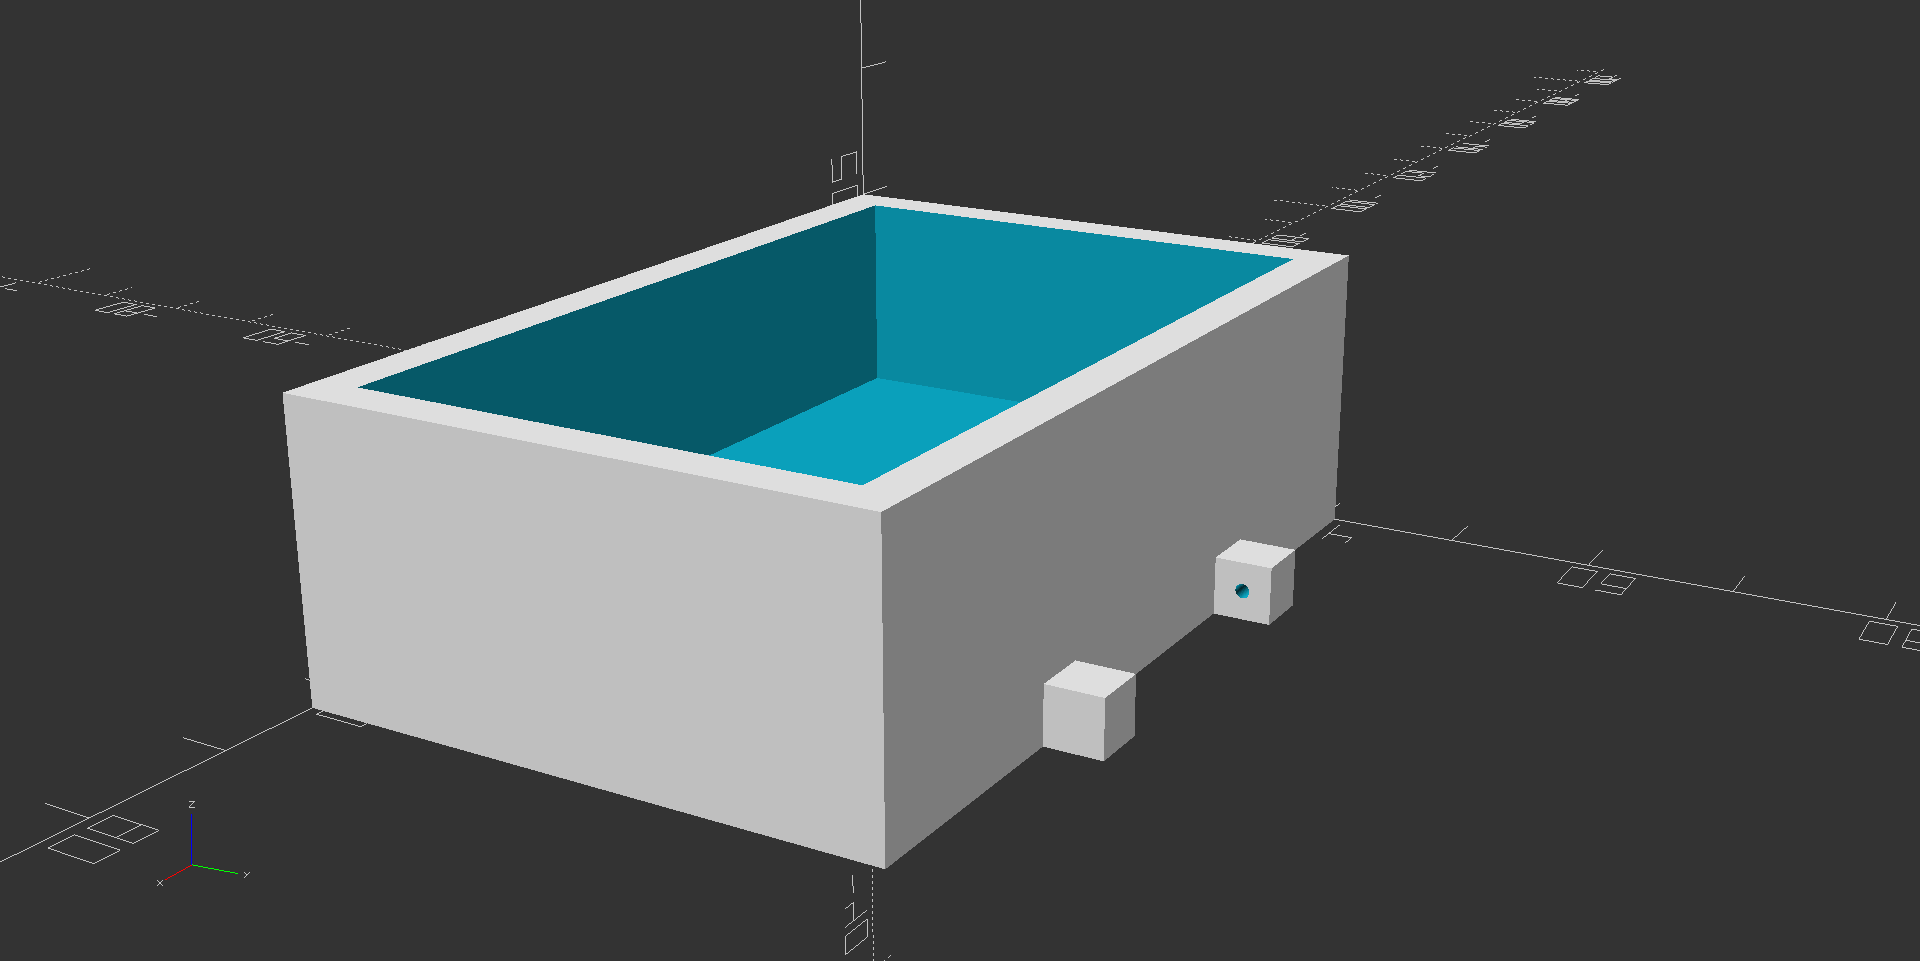
\includegraphics[width=\textwidth,height=\textheight,keepaspectratio]{images/enclosure.png}
\caption{Enclosure Render}
\label{fig:enclosure}
\end{figure}

\begin{figure}[!htb]
\centering
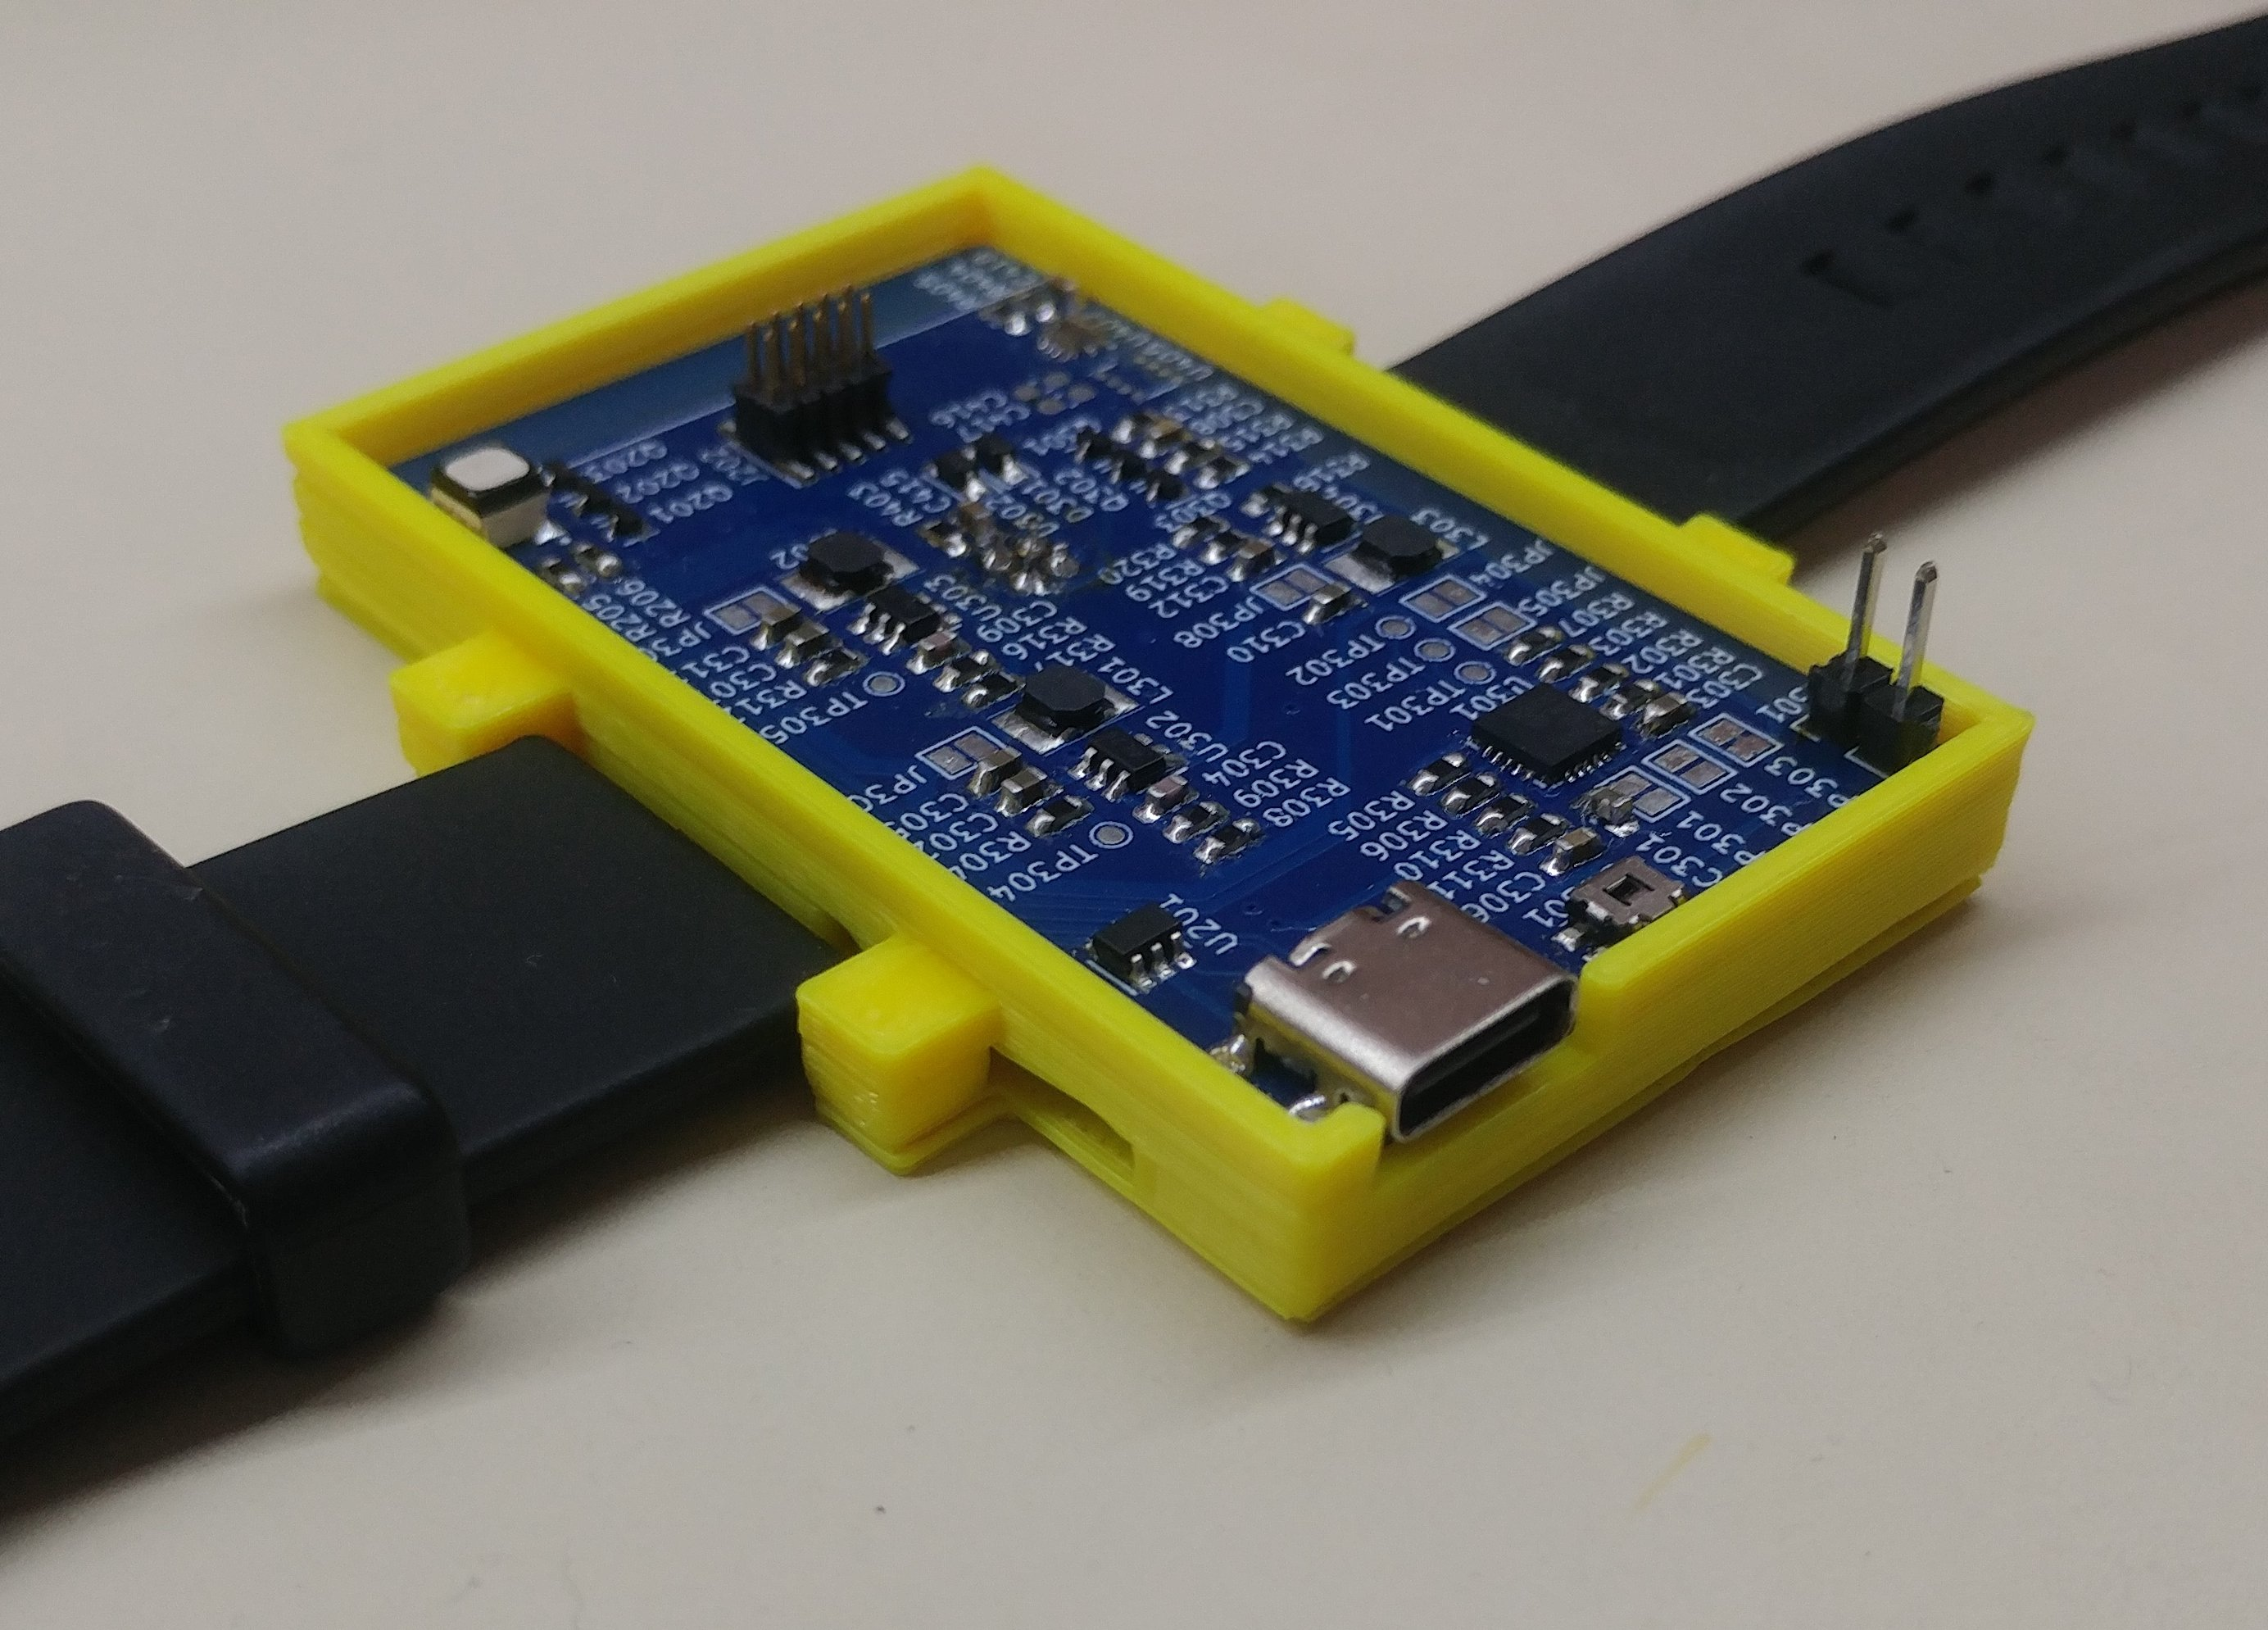
\includegraphics[width=\textwidth,height=\textheight,keepaspectratio]{images/biosense.jpg}
\caption{Fabricated Enclosure with watch straps and a board installed}
\label{fig:enclosure-fab}
\end{figure}
